%%%%%%%%%%%%%%%%%%%%%%%%%%%%%%%%%%%%%%%%%
% Modelo Latex para pôster do SBrT'24
%
% v1: Diego da Silva de Medeiros - IFSC
% v2: Leonardo Lira Ramalho - UFPA
%%%%%%%%%%%%%%%%%%%%%%%%%%%%%%%%%%%%%%%%%

%----------------------------------------------------------------------------------------
%	PACKAGES AND OTHER DOCUMENT CONFIGURATIONS
%----------------------------------------------------------------------------------------

\documentclass[a0,portrait]{a0poster}

\usepackage{multicol} % This is so we can have multiple columns of text side-by-side
\columnsep=100pt % This is the amount of white space between the columns in the poster
\columnseprule=3pt % This is the thickness of the black line between the columns in the poster
\usepackage{fancybox}
\usepackage[svgnames]{xcolor} % Specify colors by their 'svgnames', for a full list of all colors available see here: http://www.latextemplates.com/svgnames-colors

\usepackage{epsfig}
\usepackage{pdfpages}
\usepackage{cite}
\usepackage{color}
\usepackage{colortbl}
\usepackage[cmex10]{amsmath}
\usepackage{amssymb}
\usepackage{soul}
\usepackage{amsfonts}
%\usepackage{mathtools}
\usepackage[normalem]{ulem}
%\graphicspath{{fig/}}
%\usepackage{soul}
\usepackage{booktabs}
\usepackage{color}
\usepackage{placeins}
\usepackage{upgreek}
\usepackage[utf8]{inputenc}

\usepackage[export]{adjustbox}

%\usepackage{times} % Use the times font
%\usepackage{palatino} % Uncomment to use the Palatino font
\usepackage{epstopdf}
\usepackage{graphicx} % Required for including images
%\graphicspath{{figures/}} % Location of the graphics files
\usepackage{booktabs} % Top and bottom rules for table
\usepackage[font=small,labelfont=bf]{caption} % Required for specifying captions to tables and figures
\usepackage{amsfonts, amsmath, amsthm, amssymb} % For math fonts, symbols and environments
\usepackage{wrapfig} % Allows wrapping text around tables and figures
\usepackage[framemethod=TikZ]{mdframed}
\usepackage{lipsum}
\usepackage{titlesec} % Modify titles
%\usepackage{fontspec}
%\setmainfont{Calibri}
\newcommand{\ds}{\displaystyle}
\newcommand {\bo}[1]{\textbf{#1}}
\newcommand{\pa}[1]{\left({#1}\right)}
\newcommand{\co}[1]{\left[{#1}\right]}
\newcommand{\ch}[1]{\left\{{#1}\right\}}

\titleformat{\section}{\color{white}\normalfont\Large\bfseries}{\color{white}\thesection}{1em}{\colorbox{SteelBlue}}{}

\setlength{\columnseprule}{0pt}
\mdfdefinestyle{MyFrame}{%
	linecolor=SteelBlue,
	outerlinewidth=2pt,
	roundcorner=50pt,
	innertopmargin=\baselineskip,
	innerbottommargin=\baselineskip,
	innerrightmargin=20pt,
	innerleftmargin=20pt,
	backgroundcolor=white!50!white}
%\input{figconfig}
%\titleformat{command}[shape]{format}{label}{sep}{be %fore-code}{after-code}
\begin{document}
\begin{mdframed}[style=MyFrame]
%----------------------------------------------------------------------------------------
%	POSTER HEADER 
%----------------------------------------------------------------------------------------

% The header is divided into two boxes:
% The first is 75% wide and houses the title, subtitle, names, university/organization and contact information
% The second is 25% wide and houses a logo for your university/organization or a photo of you
% The widths of these boxes can be easily edited to accommodate your content as you see fit
\begin{minipage}[b]{0.33\linewidth}
\raggedright

\includegraphics[width=4cm,valign=t]{figures/minipage.png}
\end{minipage}
%
\begin{minipage}[b]{0.33\linewidth}
\centering

\includegraphics[width=20cm,valign=t]{figures/logo-ud.png}
\end{minipage}
% 
\begin{minipage}[b]{0.33\linewidth}
\raggedleft

\includegraphics[width=5cm,valign=t]{figures/minipage.png}
\end{minipage}\\

\vspace{3cm}
\begin{minipage}[h]{0.98\linewidth}
\centering \huge \color{SteelBlue} \textbf{Dental prophylaxis domain-specific LLM} \color{Black}\\ % Title
\Large \textbf{Cesar Pulido\textsuperscript{1} and Catalina Ariza\textsuperscript{2}}\\ % Author(s)
\normalsize Universidad Distrital Francisco José de Caldas\textsuperscript{1,2}\\ %[-0.5cm] % University/organization
capulidoc@udistrital.edu.co\textsuperscript{1} and catarizaa@udistrital.edu.co\textsuperscript{2}\\
\end{minipage}
\vspace{0.5cm} % A bit of extra whitespace between the header and poster content

%----------------------------------------------------------------------------------------

\begin{multicols}{2} % This is how many columns your poster will be broken into, a portrait poster is generally split into 2 columns


%----------------------------------------------------------------------------------------
%	INTRODUCTION
%----------------------------------------------------------------------------------------

\section{Introduction}\label{section:1}

Whether it's maintaining better daily cleanliness, forming healthier habits, or taking care of problems like cavities and oral diseases, dental care is a big worry for many people. Dental prophylaxis, a specialty of dentistry focusing on preventative care, plays a critical part in maintaining oral health. We are creating a chatbot to help consumers obtain fast and trustworthy solutions to their questions about dental hygiene. This chatbot will give customers expert advice on maintaining good dental health and preventing problems like cavities and gum disease, as well as pertinent information and advise on preventive actions.

Providing dental care involves a number of difficulties, particularly in teaching patients about preventative and good oral hygiene. A lot of people have trouble adopting better behaviors or treating problems like gum disease and cavities before they get worse. Ensuring the chatbot can deliver precise and trustworthy guidance catered to individual needs is one of the main research issues. Furthermore, creating a system that is easy to use and making sure the chatbot have the newest dental prophylaxis best practices is a major additional difficulty, since it guarantees users receive accurate and up-to-date information.


%
%----------------------------------------------------------------------------------------
%	OBJECTIVES
%----------------------------------------------------------------------------------------



\section{Goal}\label{section2}
%
The main question to be answered is: What is the most efficient method to achieve near-perfect oral health? Our goal is to enable people to improve their oral health by using the chat bot and to see the answer to this question.
%

\section{Technical considerations}\label{section3}

Dental prophylaxis studies both the external causes that contribute to diseases such as caries and periodontitis, including poor eating habits and the consumption of harmful substances. However, to better focus our analysis, we have decided to set aside these external causes and focus on the personal care that each person should follow, along with the procedures that the dentist performs to prevent and treat these oral diseases.

This approach allows us to concentrate on the most effective strategies for prevention and improvement of oral health from a clinical point of view.

\section{System description}\label{section4}

We define the dental prophylaxis system as having two subsystems, patient care and professional procedures. These subsystems are composed of the main cleaning elements for dental care and also procedures for it (e.g. toothbrush, dental floss, fluoride, etc). In addition to that we also define the inputs and outputs of the system (See Figure 1). 

The purpose of making this drawing is to be able to better understand the system and the relationships between its elements. This in the end will help us to make a correct analysis of the system so that people can get this information through the chatbot in the best way. 
\vspace{2cm}
\vspace{2cm}
%\hspace{1cm}
\begin{minipage}{\columnwidth}
    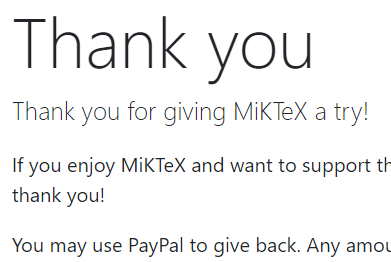
\includegraphics[width=0.9\columnwidth]{figures/fig1.png}
\end{minipage}
%\hspace{1cm}
\vspace{1cm} %\\\vspace{-10cm}


%----------------------------------------------------------------------------------------
%	REFERENCES
%----------------------------------------------------------------------------------------

%\bibliographystyle{IEEEtran}
%\bibliography{IEEEabrv,references}

%---------------------------------------------------

\end{multicols}
\begin{center}
\color{SteelBlue}{Systems Analysis - Semester 2024-III}
\end{center}
\end{mdframed}
\end{document}